% Sample Paper for Poster Conference
%( without guarantee:-)) 
%send your comment to xrund@fel.cvut.cz
%
\documentclass{poster16}
% 
%----------------------------------------------------------
%             THIS IS THE PLACE FOR YOUR FAVORITE PACKAGES
%
%\usepackage[latin2]{inputenc}%
%\usepackage{babel}% 
%\usepackage{czech}%
%\usepackage{psfrag}
%\usepackage{amsmath}
%\usepackage{pifont,amssymb}

\begin{document}
%----------------------------------------------------------

%----------------------------------------------------------
%               THIS IS THE PLACE OF THE TITLE
%
\title{3D printed rocket - platform for student experiments}
%----------------------------------------------------------
%               THIS IS THE PLACE FOR THE AUTHORS NAMES AND THE TITLE FOR HEADINGS
%
\headtitle{F. S. AUTHOR, S. S. AUTHOR, SAMPLE PAPER FOR POSTER 2016 CONFERENCE}
%----------------------------------------------------------
%               THIS IS THE PLACE FOR THE AUTHORS NAMES - ALL AUTHORS MUST HAVE A STUDENT STATUS!!!

%
\author{Jakub Kakona \affiliationmark{1}}
%----------------------------------------------------------
%              THIS IS THE PLACE FOR AFFILIATIONS
%
\affiliation{%
\affiliationmark{1}Dept. of Radio engineering, Czech Technical University, Technick\'a 2, 166 27 Praha, Czech Republic}
  \email{kakonjak@fel.cvut.cz}
%--------------------------------------------------------------


\maketitle

%----------------------------------------------------------
%               THIS IS THE PLACE FOR ABSTRACT

\begin{abstract}
The rocket sounding is known atmospheric research tool.
\end{abstract}

%----------------------------------------------------------
%               THIS IS THE PLACE FOR KEYWORDS
\begin{keywords}
Rocket experiments, 3D printing, sounding rocket, experimental platform.
\end{keywords}

%----------------------------------------------------------
%               HERE WRITE YOUR PAPER

\section{Introduction}

Scientific rocket experiments was relatively common in atmospheric research over past decades. Although the rocket sounding is similar to use of hight-altitude balloons. The rocket can reach a high altitude very quickly in well defined time window and with relatively precise coordinates. Furthermore the rocket lunch itself can be passed in relatively unfriendly weather conditions. Therefore this type of sounding has several benefits over balloon sounding. It can be used for precise in situ measurement of interesting atmospheric events. Such events could be tornado measurements, storm measurements and other usually localised but very interesting and probably dangerous processes which needs an automated measuring systems. 

Unfortunately the rocket sounding is quite inaccessible for widespread use, specifically in use as part of measurement networks. One of main reasons of that is price of the rocket lunch vehicle it is caused mainly by one-time use of relatively expensively machined device. 
As reason of that a different manufacturing and design process is needed for rocket construction. 
For appropriate range of rocket vehicles the state of the art but inexpensive FDM 3D printig process could be used. But specially designed rocket body is needed in case of use an additive manufacturing process instead of classical machining. 

\section{Design evolution}

We decided to use the Fused deposition modeling (FDM) additive manufacturing technology as best candidate for small and medium size of sounding rocket vehicle. The main reason for that decision is fact that this type of 3D printing technology is widely accessible and has quality enough to build rocket body which could windstad the mechanical and aero-dynamical stress during the rocket lunch. The second reason is fact that this type of technology is relatively  cheap in comparison of other additive manufacturing methods. 
But there also exist technological limits because not all shapes could be 3Dprinted. The problematic geometry are overhanging surfaces or large number of very small details in printed volume. 
The design of rocket vehicle therefore must have special construction which allows reliable printing without costly model specific g-code tweaking. 

\begin{figure}[ht]
\begin{center}
\resizebox{\linewidth}{!}{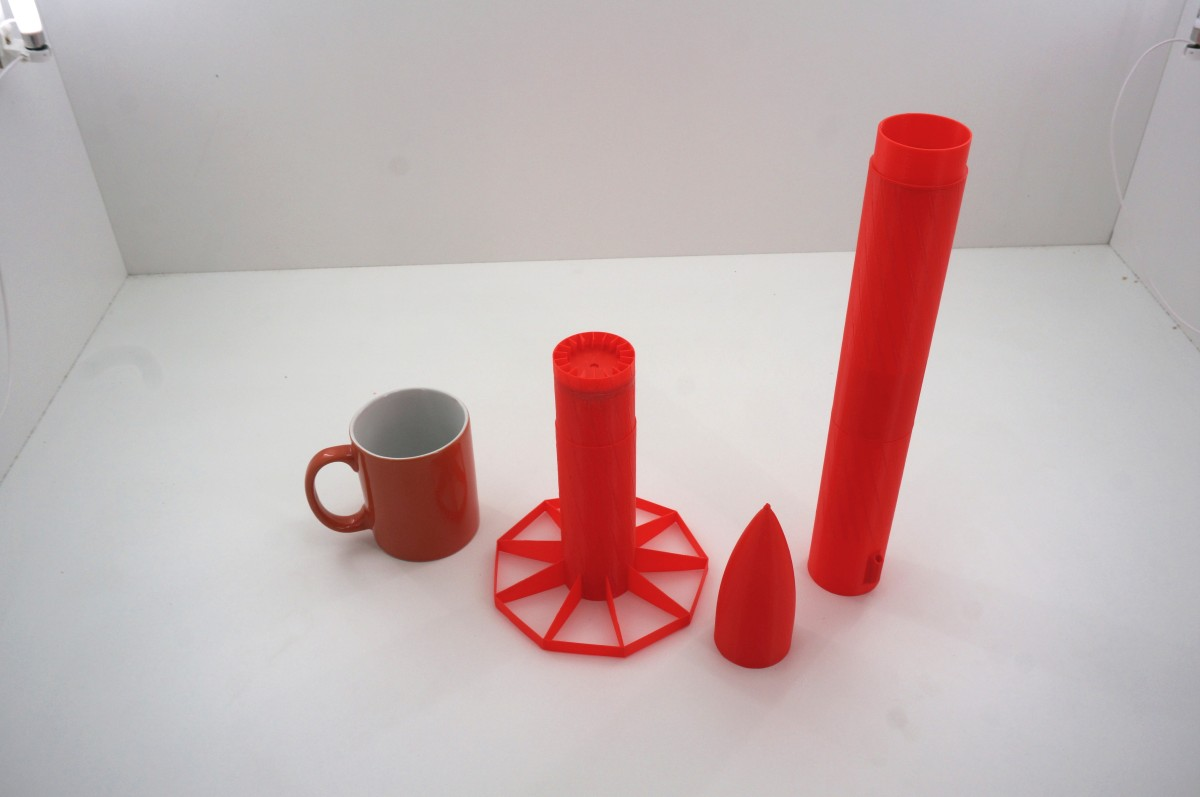
\includegraphics{./img/3dprinted_rocket_parts.jpg}}
\caption{A sample of printable rocket design. (Experimentally printed from red ABS)} 
\label{fig:printed_parts}
\end{center}
\end{figure}


\subsection{Rocket body and recovery system}

The rocket body is designed as simple as possible to minimize quality parameters requested on 3D printer used. Several mechanical construction challenging details have been resolved until a current stage of rocket development. 

\begin{itemize}
\item Fins design
\item Rocket stage connections
\item Rotket hull reinforcements
\item Reliable recovery system
\end{itemize}

The rocket fins are aero-dynamical stabilization surfaces needed for smooth stable ballistic trajectory flight.  The classical planar fins are very well known, but this type of fins in not suitable for printed model.  The long wingspan and elastic properties of PLA material tends to vibrate in high speed airflows.
Therefore alternative fins construction was considered a grid-fins design \cite{grid_fins} where the elasticity of material is very suppressed by orthogonal bonding.
Grid fins design suppose very thin wall of grid material towards to grid cross-section. This assumption significantly limits range of printable rocket sizes. The limits arise from the fact that most 3D printers have 0.4 mm nozzle diameter. Therefore extrusion width of that printer cannot be less than approximately 0.5 mm. Such grid-fin wall size cannot be used in rocket with fins wingspan smaller than approximately 7 cm. because the aero-dynamical drag of such grid fins is considerable. 

\begin{figure}[ht]
\begin{center}
\resizebox{\linewidth}{!}{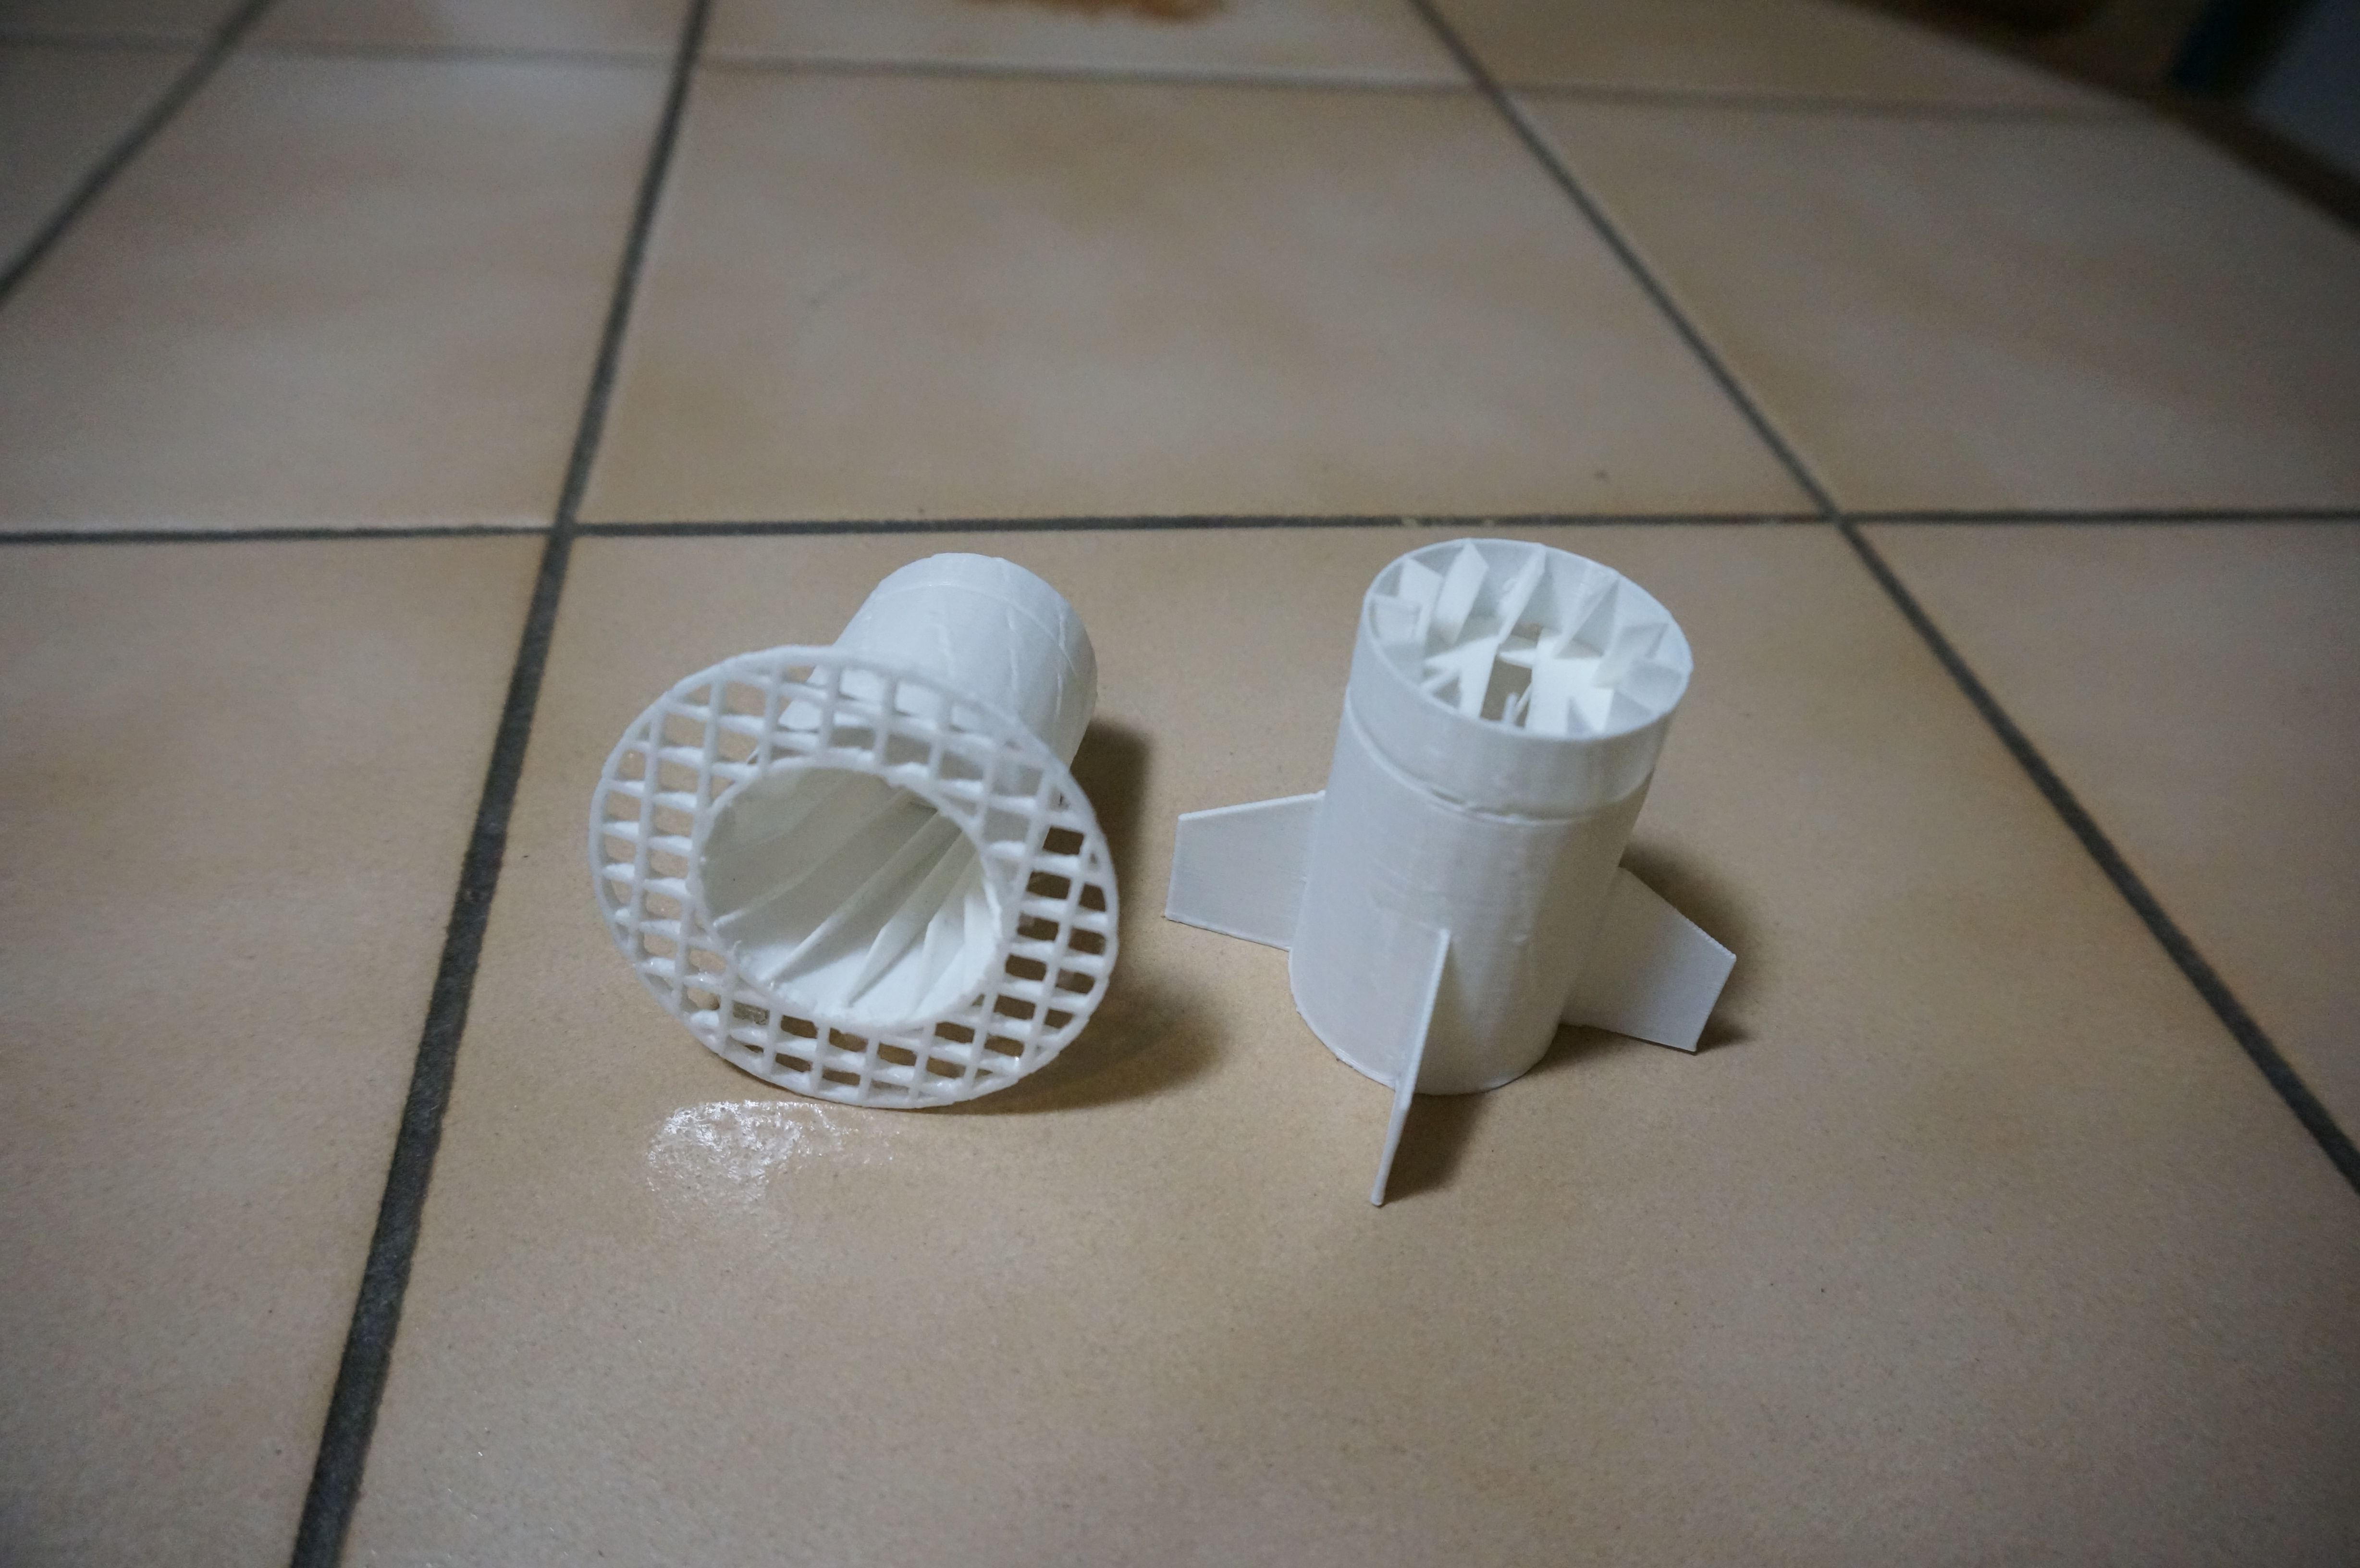
\includegraphics{./img/3d_printed_grid_fin.jpg}}
\caption{A reduced size model of grid fin based engine stage of rocket. } 
\label{fig:grid_fin}
\end{center}
\end{figure}


The drag must be reduced to achieve usable ceiling parameters. To overcome this issue a hybrid grid-fins were developed as compromise between rigidity of grid-fins and aerodynamic efficiency of classic planar fins. 


\subsection{3D printable rocket engine}

Several technical solutions were considered and tested during the rocket development. 

\begin{itemize}
\item Reusable metal case engine
\item One time use model rocket engine
\item Experiment with one time use 3D printed engine
\end{itemize}

A reusable metal engine shown in figure \ref{fig:metal_engine} was used in very first rocket design. (Which was not 3D printed really.) Testing rocket with reusable engine was lunched, but recovery was unsuccessful. The recovery system failed and rocket must be excavated from soil in the test field. Consequently the reusable rocket engine was mechanically deformed and cannot be used any more.
The reusable rocket engine was quite expensive and recovery system failure or some other system failure could not be prevented completely in future. Therefore use of reusable rocket engine was evaluated as unsuitable for experimental rocket design. 
The one time model rocket engine was used in another small but this time 3D printed design. The rocket lunch was partiality successful because the 3D printed rocket withstand the stress forces during the launch.  But parachute recovery system failed again. 

\begin{figure}[ht]
\begin{center}
\resizebox{\linewidth}{!}{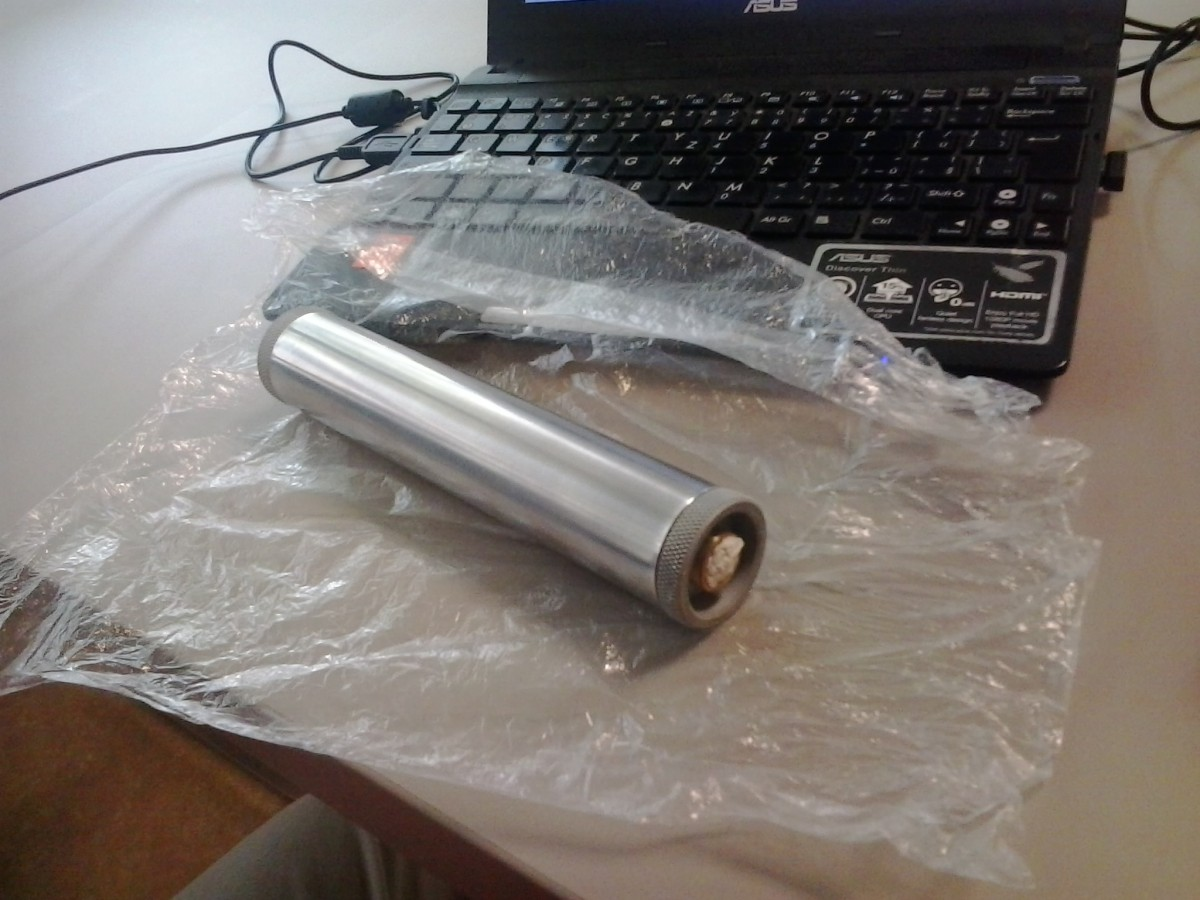
\includegraphics{./img/rocket_engine1.jpg}}
\caption{A sample of printable rocket design. (Experimentally printed from red ABS)} 
\label{fig:metal_engine}
\end{center}
\end{figure}

\section{Conclusion}






\section*{Acknowledgements}
Research described in the paper was supervised by Prof. A. Supervisor, FEE CTU in Prague and supported by the Czech Grant Agency under grant No. 102/ 01/9999, by the Czech Ministry of Education under grant No. 9999/2002 and by the research program MSM 444222.

The headline \emph{Acknowledgements} is of the  style \verb+\section*{}+.

The authors are asked to pay special attention to the form of references. The NAMES OF AUTHORS should be typed in capitals, the \emph{Titles of Journals, Books or Proceedings} in italics with the first capital letter in all significant words. The tittles of articles are typed similarly as the basic text without the first capital letter in all words. Use the standart environment \verb+thebibliography+.

%----------------------------------------------------------
%               THIS IS THE PLACE FOR REFERENCES
\begin{thebibliography}{9}
\bibitem{paper}
JAKUBOV\'A, I., RAIDA, Z. Exemplary Document for the paper in Radioengineering. \emph{Radioengineering}, 2006, vol. 15, no. 1, p. 1 - 2.
\bibitem{book}
AUTHOR, F., AUTHOR, S., AUTHOR, T. F. \emph{The Book}. 2nd ed. Humpolec: Nupish\&Publish, 1901.
\bibitem{Grid_fin}
https://en.wikipedia.org/wiki/Grid\_fin
\end{thebibliography}


%----------------------------------------------------------
%               THIS IS THE PLACE FOR AUTHOR CV
\begin{authorcv}{First AUTHOR}
was born in \dots The biography is typed using the environment \verb+authorcv{First AUTHOR}+. 

For one author, one paragraph of the biography is devoted. The \textbf{Name} of the author is typed in  \verb+\textbf{}+, the \textbf{SURNAME} is written in capitals.  All authors must have a student status!
\end{authorcv}

\end{document}

